\documentclass{article}

\usepackage{graphicx}
\usepackage{tabularx}
\usepackage{booktabs}

\renewcommand{\abstractname}{Resumen}


\title{Predicción de Diferencias de Saturación en Interacciones Proteína-Ligando}
\author{Carlos Mario Chang Jardínez\\Lidier Robaina Caraballo\\Yisell Martínez Noa\\Ernesto Rousell Zurita\\Carlos Manuel García Rodríguez}


\begin{document}
\maketitle

\begin{abstract}
    En este trabajo analizaremos distintos acercamientos para intentar predecir los STD de los atómos de un ligando en una interacción con una proteína.
    Empleamos modelos de machine learning como Random Forest, Graph Neural Network (GNNs) y técnicas de AutoML para las predicciones. La similitud entre
    los valores predichos y los experimentales es un indicador crucial: cuanto más cercanos sean, mayor será la probabi-lidad de que la pose analizada
    represente fielmente la configuración real del sistema molecular. Lo cual tendría mucha utilidad para obtener datos de sistemas moleculares más allá de
    la vía experimental que es sumamente costosa.
\end{abstract}

\newpage

\section{Introducción al problema}
Las interacciones proteína-ligando son la piedra angular del diseño racional de fármacos, pues son fundamentales en procesos biológicos como la señalización celular,
la regulación enzimática y el diseño de fármacos Estas interacciones determinan la especificidad, afinidad y estabilidad del complejo molecular, además de factores críticos
para la eficacia terapéutica. Un ligando (una molécula pequeña, un fármaco) se une a regiones específicas de una proteína mediante fuerzas no covalentes:
enlaces de hidrógeno, interacciones electrostáticas, fuerzas hidrofóbicas.

La predicción de la `pose' correcta (orientación y conformación del ligando al unirse) es crítica en drug discovery. Métodos computacionales como el docking
molecular simulan estas interacciones, pero su precisión es limitada debido a la flexibilidad conformacional y la complejidad de los entornos protéicos\cite{docking}.

La afinidad de unión (KD) se cuantifica experimentalmente mediante técnicas como ITC (Calorimetría de Titulación Isotérmica), SPR (Resonancia de Plasmón Superficial),
pero estas son costosas y lentas. Aquí, el STD-NMR emerge como una alternativa rápida para validar modelos estructurales, aunque su interpretación cuantitativa sigue
siendo un reto\cite{STD_e}.

\newpage

\section{Estado del Arte}

\subsection{STD-NMR y RedMat}
El STD-NMR es una técnica experimental que identifica regiones de un ligando en contacto directo con una proteína. Al saturar selectivamente las resonancias de la proteína,
la magnetización se transfiere al ligando unido, amplificando las señales de los protones del ligando cercanos a la superficie proteíca\cite{STD_e}. Esto permite mapear los epitopos
de interacción sin requerir purificación de la proteína o altas concentraciones de ligando.
\\
\\
Por su parte RedMat (Reduced Matrix) es un enfoque computacional que correlaciona datos de STD-NMR con modelos 3D de complejos proteína-ligando de baja afinidad, utilizando
descriptores moleculares (cargas atómicas, momentos dipolares) y los propios datos experimentales de STD-NMR. Su innovación radica en:
\begin{itemize}
    \item Algoritmo de correlación espacial: Compara las señales de STD-NMR experimentales con las predichas a partir de poses generadas por docking.
    \item Rapidez: Reduce el tiempo de validación de semanas (en experimentos tradicionales) a horas.
    \item Aplicaciones: Útil en etapas tempranas de descubrimiento de fármacos, donde se deben evaluar miles de candidatos.
\end{itemize}

\subsection{Machine Learning en Interacciones Proteína-Ligando}

Los métodos clásicos (docking con funciones de puntuación basadas en energía) suelen subestimar efectos entrópicos o solvatación. El machine learning (ML) aborda
estas limitaciones mediante:
\begin{itemize}
    \item Features: Coordenadas 3D, descriptores fisicoquímicos (logP, polaridad), fingerprints moleculares, y datos espectroscópicos (STD-NMR).
    \item Modelos: Random Forest, SVM, y redes neuronales profundas (GNNs, Transformers) para predecir afinidad o poses\cite{rf_score}.
\end{itemize}

También es posible entrenar modelos de machine learning usando datos de STD-NMR llegando a aportar algunas ventajas sobre los modelos tradicionales. Con machine learning
se es capaz de llegar a una integración multimodal donde se pueden combinar datos estructurales, descriptores y señales NMR mejora la generalización en proteínas poco estudiadas\cite{multimodal}.

\newpage

\subsection{Uso Graph Neural Network (GNNs)}
Las GNNs son ideales para modelar interacciones proteína-ligando debido a su capacidad para trabajar con datos en forma de grafos, donde los nodos representan atómos (proteína y ligando)
y las aritas pueden representar enlaces químicos o interacciones espaciales.

Las GNNs tienen algunas ventajas sobre los modelos tradicionales, como ser capaces de capturar relaciones topológicas como la polaridad local o la accesibilidad superficial mediante mecanismos
de message passing\cite{gnn}. Al igual que otros modelos de machine learning tienen la capacidad de integrar datos multimodales fusionando estructuras 3D, descriptores moleculares y señales STD-NMR\cite{nmr}. Además
de ser capaces de identificar patrones estables en las intera-cciones, incluso en conformaciones flexibles al usar poses generadas por docking.

\newpage

\section{Exploración de Datos Iniciales}

\subsection{Descripción de los datos}
Obtener datos experimentales del STD de una interacción proteína-ligando es un proceso muy costoso y por lo tanto sería muy impráctico obtener la cantidad de datos suficientes para entrenar un modelo
de machine learning. Por tanto los datos obtenidos para entrenar el modelo se formaron de la siguiente manera, usando datos experimentales de proteínas, por cada una se tomaron datos experimentales de
ligandos que reaccionan con esas proteínas, con dos técnicas diferentes se generan 200 posiciones del ligando alrededor de la proteína y se predice el STD usando RedMat. Obteniendo de esta forma más
de 10000 de estos datos.

\subsection{Preprocesamiento de los datos}
Los datos obtenidos estaban separados en tres archivos, un csv con los STD de los ligandos y sus propiedades, y dos .plb, uno con la información estructural de las proteínas y el otro el de los ligandos.
Eso llevo un preprocesamiento para poder guardar la información de una forma fácil de manejar y analizar.

\subsection{Visualización de los datos}
Aquí tenemos una pequeña muestra de los datos, donde cada fila tiene una proteína con un ligando en una posición determinada por una de las dos técnicas de posicionamiento, y varias características de cada
atómo tanto de la proteína como del ligando como coordenadas, mol, dssp, sasa. Llegando cada fila a tener hasta 400 columnas dada la cantidad de atómos
\begin{figure}[h]
    \centering
    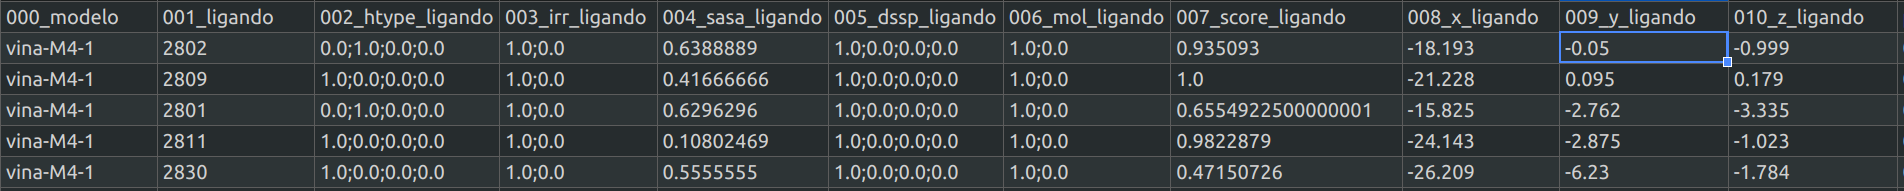
\includegraphics[width=12cm]{data_example.png}
\end{figure}

\subsection{Principales factores a tener en cuenta}
Los datos obtenidos estaban bastante bien estructurados, incluso con muchos de los valores y características ya normalizados. Se tenían 4 tipos de datos categóricos que fueron transformados usando one-hot encoder.
También teníamos vectores de diferentes tamaños ya que dependiendo de la cantidad de atómos y la posición del ligando teníamos más o menos información en cada fila.

\newpage
\section{Modelos}
Cada modelo tiene un informe más detallado adjunto junto con el código pero vamos a tocar las bases fundamentales de cada modelo.
\subsection{Modelo de grafo heterogéneo}
Se optó por entrenar sobre un grafo heterogéneo debido a su capacidad para modelar de manera más realista la estructura de los datos.
Aunque estos grafos presentan mayor complejidad en su manejo, ofrecen la ventaja de permitir la aplicación de distintas capas a cada
tipo de nodo en caso de ser necesario en futuras optimizaciones.

Dentro de nuestro grafo, se implementó una capa lineal encargada de transformar el vector de características de los nodos
(ligandos y proteínas) en un vector de tamaño variable para las capas ocultas. A continuación, se utilizaron cuatro capas HeteroConvolucionales,
encargadas de mezclar (mediante suma) las salidas obtenidas tras aplicar SAGEConv a ambos tipos de nodos.

El mecanismo de SAGEConv realiza la agregación de características en cada nodo utilizando la media de los valores de sus vecinos.
Finalmente, se añadió una última capa lineal desde la cual se extraen los valores finales de los ligandos.

Se evaluaron distintas opciones para el diseño de la arquitectura, optando finalmente por HeteroConv debido a sus ventajas en el tratamiento
de grafos heterogéneos. Para la preparación de los datos se utilizó one-hot encoding en la identificación de características como htype, irr,
dssp y mol.

\subsubsection{Experimentación con funciones de activación}
Se probaron distintas funciones de activación para optimizar el desempeño del modelo como:
\begin{itemize}
    \item ReLu
    \item ELU
    \item Swish
\end{itemize}
Inicialmente, la función Swish mostró los mejores resultados en las primeras 50 épocas. Sin embargo, se observó que, a pesar de una mejora continua
en la función de pérdida, la validación permanecía estancada. Esto sugiere que el modelo estaba aprendiendo bien los datos de entrenamiento pero sin
generalizar adecuadamente.

Para abordar este problema, se tomaron las siguientes medidas:
\begin{itemize}
    \item Aumento del número de neuronas en las capas ocultas a 100 para mejorar la capacidad de generalización.
    \item Incremento del número de épocas a 100, ya que la curva de aprendizaje, aunque errática, mostraba potencial de convergencia.
\end{itemize}
Sin embargo, estos cambios no dieron resultados significativamente mejores, lo que sugiere la necesidad de ajustar otros parámetros, como la regularización, la arquitectura del modelo o la cantidad de datos de entrenamiento.

\subsubsection{Posibles mejoras}

El entrenamiento en un grafo heterogéneo permitió modelar de manera más realista las interacciones en los datos, y la elección de HeteroConv resultó adecuada
para nuestro problema. Se realizaron diversos ajustes en la arqui-tectura y en las funciones de activación para optimizar el desempeño del modelo. Posibles mejoras
incluyen:
\begin{itemize}
    \item Normalización de las posiciones espaciales para mejorar la estabilidad del entrenamiento.
    \item Uso de embeddings posicionales para capturar mejor la estructura tridimen-sional de los datos.
    \item Ajuste de hiperparámetros adicionales, como regularización y dropout, para mejorar la generalización.
    \item Experimentación con más arquitecturas de GNN, como GATConv o GraphSAGE, para evaluar posibles mejoras en la propagación de información.
\end{itemize}


\subsection{AutoML}

Este proyecto utiliza Auto-sklearn, una herramienta de Auto Machine Learning (AutoML), para predecir los valores de STD en una base de datos que contiene información
sobre proteínas y ligandos. El objetivo es encontrar el mejor modelo para realizar predicciones precisas a partir de las características extraídas.

Se han realizado varias configuraciones de entrenamiento con distintos tiem-pos de entrenamiento, tamaños de ensamble, estrategias de validación y manejo de
valores faltantes, con el fin de optimizar el rendimiento del modelo.


\subsubsection{Análisis de las configuraciones}
En la mayoría de los experimentos, Gradient Boosting (HistGradientBoostingRegressor) fue el modelo dominante, lo que indica que es la mejor opción para estos datos.
Otras técnicas como KNN y Decision Trees solo aparecen cuando se desactiva el metalearning. Probar diferentes estrategias de manejo de valores faltantes no
tuvo un gran impacto en los resultados, lo que indica que el método de imputación de AutoML ya estaba funcionando bien.

\subsubsection{Posibles mejoras}
\begin{itemize}
    \item Optimización manual de hiperparámetros de Gradient Boosting para mejorar aún más el rendimiento.
    \item Explorar ajustes en el ensamble para diversificar los modelos usados.
    \item Probar técnicas de selección de características para reducir la dimensionalidad.
\end{itemize}

\subsection{Random Forest Regressor}
Se creó un modelo de random forest usando sklearn. Para el Preprocesamiento de datos de este modelo en particular se eliminó las columnas más del 80\% de los datos
vacíos para resolver el problema de los vectores de diferentes tamaños. Usando un total de 100 árboles sin especificar la profundidad de cada árbol. La cantidad de
muestras requeridas en cada hoja fue de 5 y la cantidad de muestras requeridas para dividir un nodo fue de 2. Estas configuraciones fueron las que mejores resultados
alcanzaron.


\newpage

\section{Análisis de métricas y resultados}
Las métricas más usadas en estos modelos fueron las siguientes:
\begin{itemize}
    \item \(R^2\): Representa la proporción de la varianza que puede ser explicada por las variables independientes en el modelo.
          \(R^2(y,y')= 1 - \sum\frac{(y_i-y'_i)^2}{(y_i- \bar{y})^2 }\)
    \item Error absoluto medio: \(MAE(y,y')= \frac{1}{n} \sum |y_i-y'_i|\)
    \item Error cuadrático medio: \(MSE(y,y')= \frac{1}{n} \sum (y_i-y'_i)^2\)
\end{itemize}

Enfocándonos sobre todo en el error medio absoluto (MAE) por ser una representación más entendible y real de cuanta diferencia había
entre las predi-cciones y valores reales, pudiendo consultar a expertos del tema cuanto error es admisible por el modelo para que sea
considerado bueno. Y en el \(R^2\) para ver que tanto explican las variables del comportamiento real.

\subsection{Resultados de cada modelo}
\subsubsection{Grafo heterogéneo}
Además de las métricas antes mencionadas en este modelo se aplicó también K-Fold Cross Validation.

La validación cruzada de K pliegues es una técnica que permite evaluar la capacidad de generalización de un modelo. En lugar de
dividir el conjunto de datos en solo dos partes (entrenamiento y prueba), se divide en K subconjuntos (o “folds”) de tamaño similar.
Luego, el modelo se entrena y evalúa K veces, utilizando cada fold una vez como conjunto de validación y los \(K-1\) folds restantes como
conjunto de entrenamiento.

Ventajas de K-Fold Cross-Validation:
\begin{itemize}
    \item Mejor estimación del rendimiento: Se obtiene una estimación más robusta y confiable del desempeño del modelo en comparación con una sola división de datos.
    \item Uso eficiente de los datos: Cada dato se emplea tanto para entrenamiento como para validación, lo que es especialmente útil en conjuntos de datos pequeños.
    \item Detección de sobreajuste: Si el modelo muestra una variabilidad significa-tiva en los resultados de cada fold, podría estar sobreajustando a los datos.
\end{itemize}


\newpage

El mejor resultado que se obtuvo con este modelo fue con 60 de época, con la función de activación swish, y 30 neuronas en las capas ocultas. A continuación podemos ver una
gráfica de este resultado:

\begin{figure}[h]
    \centering
    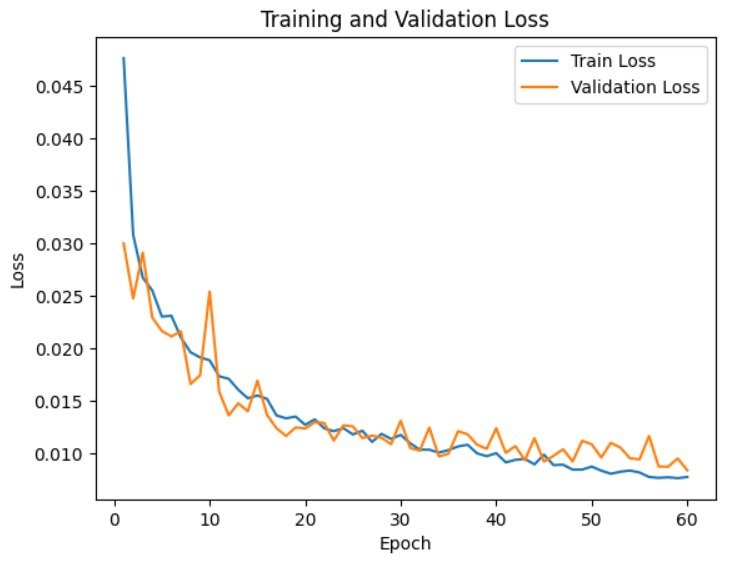
\includegraphics[width=12cm]{result.jpg}
\end{figure}

Y con los siguientes resultados a las métricas:
\begin{itemize}
    \item MSE: 0.0096,
    \item MAE: 0.0748,
    \item \(R^2\): 0.8465
\end{itemize}

\newpage

\subsubsection{AutoML}
En la siguiente tabla mostramos cada configuración con la que se corrió el algoritmo de AutoML y que resultados arrojó.


\begin{table}[h]
    \centering
    \small % Reduce el tamaño de la fuente
    \renewcommand{\arraystretch}{1.2} % Espaciado entre filas
    \begin{tabularx}{\textwidth}{|c|c|c|c|X|X|}
        \hline
        \textbf{Exp.} & \textbf{MSE ↓}  & \textbf{MAE ↓}  & \textbf{R² ↑}   & \textbf{Mejor modelo}                                             & \textbf{Observaciones}                                \\
        \hline
        1             & \textbf{0.0143} & 0.0920          & \textbf{0.7786} & \textbf{Gradient Boosting (98\%) + Extra Trees (2\%)}             & Solo encuentra \textbf{Gradient Boosting}             \\
        \hline
        2             & \textbf{0.0135} & \textbf{0.0900} & \textbf{0.7903} & \textbf{Gradient Boosting}                                        & Sigue favoreciendo \textbf{Gradient Boosting}         \\
        \hline
        3             & \textbf{0.0133} & \textbf{0.0893} & \textbf{0.7939} & \textbf{Gradient Boosting}                                        & Aumentar tiempo mejora el rendimiento ligeramente     \\
        \hline
        4             & \textbf{0.0139} & \textbf{0.0911} & \textbf{0.7841} & \textbf{Gradient Boosting}                                        & Eliminación de columnas no impactó significativamente \\
        \hline
        5             & \textbf{0.0139} & \textbf{0.0914} & \textbf{0.7840} & \textbf{Gradient Boosting}                                        & Uso de valor extremo para faltantes no afectó mucho   \\
        \hline
        6             & \textbf{0.0209} & \textbf{0.1139} & \textbf{0.6766} & \textbf{KNN (55\%) + Decision Tree (40\%) + ARD Regression (5\%)} & \textbf{Sin metalearning favorece más modelos}        \\
        \hline
    \end{tabularx}
    \caption{Resultados de experimentos con diferentes modelos de predicción}
    \label{tab:resultados_experimentos}
\end{table}

\subsubsection{Random Forest}
Los resultados a las métricas evaluadas fueron:
\begin{itemize}
    \item MSE: 0.0148,
    \item MAE: 0.0962,
    \item \(R^2\): 0.7701
\end{itemize}

\newpage

\section{Conclusiones}

El modelo que hizo un mejor trabajo prediciendo fue el de grafo heterogéneo con una MAE de 0.0748 que según un experto es una medida buena pero no lo suficiente como para ser perfecta o guía en este ámbito.

Cabe destacar que con más tiempo para obtener datos por los medios que antes mencionamos mejoraría la eficacia de los modelos. Y que a medida que se sigan haciendo datos experimentales sobre proteínas
y ligandos podríamos agrandar mucho más los datos con información real.

Es importante tener en cuenta que los datos de proteínas y ligandos son experimentales pero los valores STD y las posiciones de los ligandos son generados por la matriz de relajación que es otro modelo,
si en un futuro se volviera más sencillo generar datos de STD experimentales se podría reentrenar el modelo para que su precisión fuera mayor. Si se dieran esas condiciones es posible que se podría entrenar
un modelo para alcanzar un MAE de menos de 0.03 lo cuál seria perfecto para usar para predecir valores STD reales.

\newpage

\bibliographystyle{plain}
\bibliography{biblio}



\end{document}